\cotefile{76}
\scanpage{33}
donné par $\sigma^{\unsure{\ast|\alpha}}=i_{B,A}^{\ast}$. \unsure{Quand|Faisant} varie $A$ dans $\mathrm{Pf}_{\unsure{n+1|n-1|m+1}}(\mathbb N)$, on trouve
\[ \sigma^{\ast}\colon \Theta_m(D)\unsure{\text{---}|\longrightarrow}\Theta_n(D) \]
avec transitivité évidente. Donc les $\Theta_n(D)$ $(n\in\mathbb N)$ forment un ens. quasi simplicial (op. simpliciales définies pour applications \uline{str$^{t}$. croissantes}) i.e. définissent un foncteur
\[ \underset{\substack{\text{ens. finis tot}^{\mathrm t}\\\text{ordonnés, avec}\\\text{appl. str. cr.}}}{\left(\frac12\mathrm{Simpl}^{\ast}\right)^{\circ}}\longrightarrow(\mathrm{Ens}) \]

[ Tout ceci marche en remplaçant $\mathbb N$ par un ens ordonné quelconque \inserted{$N$}, $\mathrm{Pf}(\mathbb N)$ par l'ens \inserted{$\mathrm{Dr}(N)$} des parties finies tot$^{t}$ ordonnées de $N$, i.e. l'ens des drapeaux de $N$, qui est aussi l'ens ordonné associé \deleted{au} \inserted{à la cat. fibrée définie par le} foncteur
\[ \left(\frac12\mathrm{Simpl}^{\ast}\right)\xrightarrow{\varphi_N}\mathrm{Ens} \]
donné par
\[ \varphi_N(\Delta_n)=\mathrm{Mon.}\,\mathrm{croiss}\,(\Delta_n,N) \]
\diagram{\begin{tikzcd}[ampersand replacement=\&]\mathrm{Dr}(N)\arrow[d, "{\text{--- appl. str. croissantes}}"]\\\frac12\mathrm{simpl}\end{tikzcd}}
% archive sheet number: 32
\scanpage{34}
On a alors, \deleted{des applications \unsure{str. décroiss.|str. croiss.}} \inserted{pour un \unsure{contrafoncteur}}
\[ D\colon \underline{\mathrm{Dr}(N)}^{\circ}\longrightarrow\mathrm{Ens}, \]
définissant une catégorie fibrée sur $\underline{\mathrm{Dr}(N)}$ associée \unsure{:|à} un ens ordonné $\Theta(D)$, une appl. strictement croissante $\Theta(D)\unsure{\text{---}|\to}\mathrm{Dr}(N)$, d'où appl. composée
\diagram{\begin{tikzcd}[ampersand replacement=\&]\Theta(D)\arrow[d]\\\mathrm{Dr}(N)\arrow[d]\\\left(\frac12\mathrm{Simpl}\right)^{\ast}\end{tikzcd}}
% archive sheet number: 33
\scanpage{36}
\margin{\deleted{\unsure{Drapeaux|Divers}} Cartes cellulaires $n$-dim et groupes cartographiques.}
\[ X_{-1}=\varnothing\subset X_0\subset X_1\subset\cdots\subset X_{n-1}\subset X_n=X\qquad\text{``filtration \(n\text{-}\)admissible''} \]
a) \inserted{(\unsure{si|pr|pour} $0\leq i\leq n$)} $\mathrm{Déc}\,(X_i,X_{i-1})\inserted{=\widetilde X_i}$ est \deleted{une réunion disjointe} \inserted{somme top} de boules \inserted{fermées} de dim $i$, dont la partie marquée $\unsure{L_i|Z_i|\Xi_i}$ (image inverse de $X_{i-1}$ par $\widetilde X_i\to X_i$) est le bord
\diagram{\begin{tikzcd}[ampersand replacement=\&,column sep=small]\widetilde X_i\arrow[d,"{\unsure{\mathrm{pr}|p_i}}"']\&[-1em]\supset\&[-1em]\partial\widetilde X_i\arrow[d,"{q_{i-1}}"]\\X_i\&\supset\&X_{i-1}\end{tikzcd}}
($\Rightarrow X_i-X_{i-1}$ est une \deleted{\unsure{réunion}} somme top. de boules ouvertes de dim $i$), enfin $\widetilde X_i\to X_i$ est un morphisme fini.
b) \inserted{(\unsure{si|pr|pour} $1\leq i\leq n$)} La filtration sur $\partial\widetilde X_i$ image inverse de la filtration \deleted{de} $\varnothing\subset X_0\subset X_1\subset\cdots\subset X_{i-1}$ est \inserted{$(i-1)$-}admissible (\uline{NB} le cas $\unsure{v|i}=1$ est trivial), et les applications $q_i^{-1}(X_j)-q_i^{-1}(X_{j-1})\to X_j-X_{j-1}$ $(0\leq j\leq i-1)$ sont étales.

Ceci donne une définition récurrente de ``filtration $n$-admissible'' pour $n\geq 0$
\deleted{\(\left\{\begin{aligned}&\text{filtration \(n\)-admissible}\ \Longleftrightarrow\\ &(\varnothing\subset X_0\subset\cdots\subset X_{n-1})\ \text{est \(n-1\)-admissible,}\\ &\widetilde X_n\ \text{\unsure{somme top.} de \(n\)-boules fermées}\ldots\end{aligned}\right.\)}
\textcircled{0} Filtration $0$-admissible \qquad $\varnothing\subset X_0=X$ : $X$ discret (néc. et \uline{suffisant} par déf.)
\textcircled{1} \qquad --- \qquad $1$-admissible \qquad $\varnothing\subset X_0\subset X_1$
$X_0$ discret, $\mathrm{Déc}(X_1,X_0)\inserted{=\widetilde X_1}$ somme top. de segments, \unsure{sa|dont} partie marquée est $\partial\widetilde X_1$, et $\widetilde X_1\unsure{\text{---}|\to}X_1$ propre.
\[ \Longleftrightarrow (X_0,X_1)\ \text{\unsure{1-complexe|un complexe} top} \]
\ldots

Filtration $n$-admissible : se déduisent de filtration $(n-1)$-admissible
\[ \varnothing\subset X_0\subset X_1\subset\cdots\subset X_{n-1} \]
en attachant à $X_{n-1}$ un esp. $\widetilde X_n$ réunion disjointe de $n$-boules fermées, par une application continue \uline{finie} $\partial\widetilde X_n\overset{q_n}{\unsure{\text{---}|\longrightarrow}}X_{n-1}$ telle que l'image inverse de la filtration donnée de $X_{n-1}$ soit une filtr. $n$-admissible de $\partial\widetilde X_n$, et
% archive sheet number: 35
\scanpage{37}
donne lieu à des applications \uline{étales}
\[ q_n^{-1}(X_i)-q_n^{-1}(X_{i-1})\unsure{\text{---}|\to}X_i-X_{i-1}\qquad(0\leq i\leq n-1) \]

Morphisme d'espaces à $n$-filtrations régulières
\diagram{\begin{tikzcd}[ampersand replacement=\&,row sep=0.1em]f\colon X\arrow[r]\&Y\\[-.4em]\rotatebox{90}{$=$}\&\rotatebox{90}{$=$}\\X_n\&Y_n\\\rotatebox{90}{$\subset$}\&\rotatebox{90}{$\subset$}\\\vdots\&\vdots\end{tikzcd}}
a) $f$ fini
b) $f^{-1}(Y_i)=X_i$ \qquad $(0\leq i\leq n)$
c) $\deleted{\unsure{\forall i|f_i}}.\ X_i-X_{i-1}\unsure{\text{---}|\to}Y_i-Y_{i-1}$ est étale (donc un rev. étale)
% slanted
\margin{\uline{NB} $X_n\mapsto X_i$, $X_n\mapsto\deleted{\unsure{\partial}}\widetilde X_i$, $X_n\mapsto\partial\widetilde X_i$ sont des foncteurs de $\unsure{\mathcal F_n|F_n}$ dans $\mathcal F_i$, $\unsure{\mathcal F_i|\mathcal F_{i-1}}$, \deleted{$\unsure{\mathcal F_i}$} $\mathcal F_{i-1}^{\circ}$ resp. (\unsure{après vérification|vérifiant}). $\partial\widetilde X_i\to X_{i-1}$ \unsure{hom fonctoriel|homéomorphe}\ldots}

Catégorie $\mathcal F_n$ des espaces à $n$-filtrations régulières ss-catégorie pleine \deleted{\unsure{de}} $\mathcal F_n^\circ$ des \deleted{esp} $n$-variétés à $n$-filtr. régulière.

$G_n$ grpe $n$-cartographique (engendré par $\sigma_0\,\sigma_1\ldots\sigma_n$
\[ \begin{aligned}&\text{avec }\sigma_i^2=1\qquad(0\leq i\leq n)\\ &\sigma_i\sigma_j=\sigma_j\sigma_i\quad\text{si }n\geq j\geq i+2,\ i\geq0\\ &\deleted{\unsure{\Longleftrightarrow}}\quad\text{(condition si }n\deleted{\unsure{>}}\geq2) \end{aligned} \]

Par récurrence sur $n$, on va définir des foncteurs
\diagram{\begin{tikzcd}[ampersand replacement=\&]\mathcal F_n^\circ\arrow[r,"E_n^\circ"]\&G_n\text{-ens}\arrow[d,"\text{oubli}"]\&(\uuline{$n\geq1$})\\[-.4em]\rotatebox{90}{$\supset$}\&{}\&{}\\[-.5em]\mathcal F_n\arrow[r,"E_n"]\&G_{n-1}\text{-ens}\&{}\end{tikzcd}}
\diagram{\begin{tikzcd}[ampersand replacement=\&,column sep=small]\widetilde X_1\arrow[d,"{\unsure{p_0|p_1}}"']\&\supset\&\widetilde X_0\arrow[d,"q_0"]=\partial\widetilde X_1\\X_1\&\supset\&X_0\end{tikzcd}}
\textcircled{1} Cas $n=1$ \qquad $\unsure{E_n^\circ|E_n}(X_1)=\pi_0(\underbrace{\widetilde X_1^{\mathrm{or}}}_{\substack{\text{rev. orienté}\\\text{de }\widetilde X_1}})={}$ ens des arcs de $X_1$ $=\partial\widetilde X_1$
\deleted{= \unsure{ensemble, couples} $(\unsure{a_0,a_1}),\ldots$} \deleted{$\sigma_0$ = changement d'orientation} \deleted{\illegible{1}} \deleted{$\unsure{\sigma_1(x)}$}
\deleted{$a_0\in\partial\widetilde X_1,\ a_1\in\pi_0(\widetilde X_1),\ a_0\in a_1$}
\figure{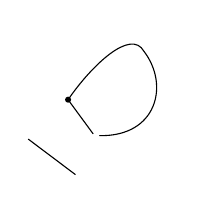
\begin{tikzpicture}[scale=.55]\fill (0,0) circle(.07);\draw (0,0).. controls (.55,.8) and (1.45,1.65) .. (1.75,1.12).. controls (2.35,.34) and (2.05,-.86) ..(.72,-.83);\draw (.58,-.79)--(0,0);\draw (-.92,-.91)--(.17,-1.73);\end{tikzpicture}}
\deleted{$\sigma_0={}$ chg$^{t}$ d'orientation} \deleted{échangeant les p$^{\rm ts}$ des fibres de} \deleted{\unsure{la projection} $\unsure{\sigma_1(a_0,a_1)=(a'_0,a_1)}$} \deleted{$a'_0\ne a_0$}
\deleted{$F_n^\circ(X_1)=\partial\widetilde X_1\to\pi_0(\partial\widetilde X_1)$} \deleted{$\sigma_1(a_0)\unsure{=}(a'_0\unsure{,a'_1})$ avec $q_0(a_0)=q_0(a'_0)$ $a'_0\ne a_0$} \deleted{$q_0(a_0)=q_0(a'_0)$} \deleted{échange les p$^{\rm ts}$ des fibres de $\partial\widetilde X_1\to X_0$}
% archive sheet number: 36
\scanpage{38}
(avec diagramme commutatifs).

\textcircled{1} $n=1$ \qquad On pose pour $X_1\in\mathrm{Ob}\,\unsure{\mathcal F_n|F_n}$
\[ E_1(X_1)=\partial\widetilde X_1\simeq\underset{\substack{\rotatebox{90}{$=$}\\\mathrm{arcs}(X_1)}}{\pi_0(\partial\widetilde X_1)}\deleted{\unsure{\sim|=}}\longrightarrow\pi_0(\widetilde X_1) \]
Les fibres de ce morphisme sont toutes de cardinal 2, d'où \deleted{\unsure{fonction}} \inserted{permutation} $\sigma_0$ commutant à ce morphisme, ss pt fixe (``permutation caractéristique'' de ce morphisme). Si $X_1$ est une $1$-variété, l'appl.
\diagram{\begin{tikzcd}[ampersand replacement=\&]E_1(X_1)=\partial\widetilde X_1\arrow[d]\\X_0\end{tikzcd}}
a\deleted{\unsure{st}} aussi ses fibres de card. 2, \deleted{\unsure{la}} perm. car. sera notée $\sigma_1$

\textcircled{2} Cas $n\geq2$. On pose
\[ E_n(X_n)=E_{n-1}^\circ(\partial\widetilde X_n)\qquad(=E_{n-1}(\partial\widetilde X_n)) \]
Muni des $\sigma_0,\text{---},\sigma_{n-1}$ i.e. op. de $G_{n-1}$ par hyp. de récurrence. Fonctorialité évidente, \inserted{comme composé de foncteurs $\mathcal F_n\xrightarrow{\partial\widetilde{\phantom X}}\mathcal F_{n-1}^\circ\xrightarrow{E_{n-1}^\circ}(G_{n-1}\text{-ens})$}
Si $X_n$ est une $n$-variété, \deleted{\unsure{critère}} \inserted{l'application}
\diagram{\begin{tikzcd}[ampersand replacement=\&] E_{n-1}(\partial\widetilde X_n)\arrow[d]\\E_{n-1}(X_{n-1})\end{tikzcd}}
% slanted
\margin{vérifier}
(c'est \unsure{une|un} $G_{n-2}$-hom, i.e. commute à $\sigma_1\ldots\sigma_{n-2}$) a des fibres de cardinal 2, l'hom can. \deleted{\unsure{ass.}} noté $\sigma_n$, il commute à $\sigma_1,\ldots,\sigma_{n-2}$. OK.
Fonctorialité claire encore ds $\mathcal F_n^\circ$
% archive sheet number: 37
\scanpage{39}
\uline{Th. 1} \inserted{Soit $n\geq1$.} Le foncteur $E_n^\circ$ passe à la catégorie isotopique $f_n^\circ$, et induit un foncteur \uuline{pl. fidèle}
\[ f_n^\circ\longrightarrow(G_n\text{-ens}) \]
(dont l'image essentielle est formée des $G_n$-ens. tels que les $\sigma_i$ $(0\leq i\leq n)$ \inserted{y} opèrent \deleted{sans pts fixes} \inserted{librement}.

Considérons $X_n\in\mathrm{Ob}\,\mathcal F_n$. On lui associe une cascade d'ens. à opérateurs
\diagram{$\begin{array}{lll} R_n(X_n)\overset{\mathrm{dfn}}{=}E_n(X_n)=\unsure{1|I}&G_{n-1}\text{-ens}&\sigma_0\ldots\sigma_{n-1}\\ R_{n-1}(X_n)=E_{n-1}(X_{n-1})&G_{n-2}\text{-ens}&\sigma_0\ldots\sigma_{n-2}\\ \ldots&&\\ R_1(X_n)=E_1(X_1)&G_0\text{-ens}&\sigma_0\\ R_0(X_n)=E_0(X_0)\overset{\mathrm{dfn}}{=}X_0&G_{-1}\ \text{ens}&\text{i.e. ensemble}\end{array}$}
De plus on a \deleted{\unsure{de}} \deleted{\unsure{des appl.}} \inserted{une} cascade d'applications
\[ R_n(X_n)\to R_{n-1}(X_n)\to\ldots\to R_0(X_n) \]
\deleted{\unsure{définie|définies}}
\diagram{\begin{tikzcd}[ampersand replacement=\&,row sep=.15em]R_i(X_n)\arrow[r]\&R_{i-1}(X_n)\&\text{hom de }G_{i-2}\text{-ens}\\\rotatebox{90}{$=$}\&\rotatebox{90}{$=$}\&\text{(commute à}\\E_i(X_i)\&E_{i-1}(X_{i-1})\&\sigma_0\ldots\sigma_{i-2})\\\rotatebox{90}{$=$}\&{}\&{}\\E_{i-1}^\circ(\partial\widetilde X_i)=E_{i-1}(\partial\widetilde X_i)\&{}\&{}\end{tikzcd}}
se déduit de $\partial\widetilde X_i\unsure{\text{---}|\to}X_{i-1}$ \unsure{en|par} appliquant le foncteur $E_{i-1}$.

\uline{Th 2} \inserted{Soit $n\geq0$.} Soit $(\mathrm{Casc}_n)$ la catégorie des ``cascades d'ens à op'' sous les grpes $G_{\unsure{n-1|n+1}},G_n,\ldots,G_0$, $G_{-1}=\{1\}$, on a donc un foncteur
% archive sheet number: 38
\scanpage{40}
\[ \underset{\substack{|\\\text{catégorie isotopique}\\\text{déduite de }\mathcal F_n}}{\unsure{f_n|\mathfrak f_n}}\xrightarrow{\varphi_n}(\mathrm{Casc})_n \]
Ce foncteur est pl. fidèle.

Il faut encore trouver \deleted{le} \inserted{un} foncteur \deleted{(\unsure{défini à iso unique}.}
\[ \deleted{\unsure{G_n}}\quad(G_n\text{-ens})\overset{\unsure{\rho_n|\varphi_n|\psi_n}}{\unsure{\text{---}|\longrightarrow}}(\mathrm{Casc})_n \]
rendant commutatif le diagramme
\diagram{\begin{tikzcd}[ampersand replacement=\&] f_n^\circ\arrow[r,hook]\arrow[d,hook]\&(G_n\text{-}\mathrm{ens})\arrow[d,"{\deleted{\unsure{E}}\rho_n}"]\\ f_n\arrow[r]\&(\mathrm{Casc})_n\end{tikzcd}}
Soit donc $X_n\in\mathrm{Ob}\,\mathcal F_n^\circ$
\uline{Th. 3}
\[ \left\{\begin{aligned} R_n(X_n)&\simeq E_n^{\unsure{\circ|\ast}}(X_n) && G_{n-1}\text{-ens}\quad\substack{\text{(NB. on a}\\\text{oublié l'opération }\sigma_n)}\\ R_{n-1}(X_n)&\simeq E_n^\circ(X_n)/\sigma_n && G_{n-2}\text{-ens}\\ R_{n-2}(X_n)&\simeq E_n^\circ(X_n)/(\sigma_n,\deleted{\unsure{\sigma}}\sigma_{n-1}) && G_{n-3}\text{-ens}\\ &\vdots\\ R_1(X_n)&\simeq E_n(X_n)/(\sigma_n,\ldots,\sigma_2)\\ R_0(X_n)&\simeq E_n(X_n)/(\sigma_n,\deleted{\unsure{\sigma}}\ldots,\sigma_2,\sigma_1) \end{aligned}\right. \]
\margin{$\checkmark$}
avec morphismes de transition définis par passage au quotient sans plus
% archive sheet number: 39
\scanpage{41}
On voudrait trouver des foncteurs (adjoints ?) en sens inverse
\diagram{\begin{tikzcd}[ampersand replacement=\&,row sep=small]\unsure{f_n^\circ|\mathfrak f_n^\circ}\&G_n\text{-ens}\arrow[l]\arrow[dd,dashed]\\\rotatebox{90}{$\supset$}\&{}\\f_n\&(\mathrm{Casc})_n\arrow[l,"\psi_n"]\end{tikzcd}}
On définira $\psi_n$ par récurrence sur $n$.

\textcircled{1} $n=0$ \qquad $\psi_0(E_0)=E_0$ avec top. discr.
\textcircled{2} Cas général.
\[ \overbrace{E_n\to\underbrace{\overbrace{E_{n-1}\to\ldots\to E_1\to E_0}^{C_{n-1}}}_{\substack{\text{définit }X_{n-1}\supset X_{n-2}\supset\ldots\\\text{par hyp. de réc.}\\X_{n-1}=\unsure{\varphi_{n-1}|\psi_{n-1}}(C_{n-1})}}}^{C_n} \]
On aura \quad $\pi_0(\widetilde X_n)\simeq E_n/G_{n-1}$
$\partial\widetilde X_n$ est défini par \deleted{\illegible{1}} ($E_n$ avec action de $G_{n-1}$) par l'hyp. de récurrence
\[ \begin{aligned} \deleted{\unsure{\partial}}X_{n-1}&=\psi_{n-1}(C_{n-1})\\ \partial\widetilde X_n&=\psi_{n-1}(\rho_{n-1}(E_n)) \end{aligned} \]
$\partial\widetilde X_n\to X_{n-1}$ déduit en appliquant $\psi_{n-1}$ à
\[ \rho_{n-1}(E_n)\longrightarrow C_{n-1} \]
\margin{préciser ce point}

Donc on définira
\[ \psi_n(C_n)=\text{\deleted{\unsure{Cône}} \inserted{Multicône} de }\psi_{n-1}\bigl(\rho_{n-1}(E_n)\to C_{n-1}\bigr) \]
\textemdash\,\textemdash\,\textemdash\quad Il faudrait donc expliciter en un \uline{Th 4} Description de $\psi_n\colon(\mathrm{Casc})_n\to\mathcal F_n$, et le cas échéant propriété d'adjonction.
% archive sheet number: 40
\scanpage{42}
Enfin, on devrait donner un
\uline{Th. 5} Subdivision barycentrique de $\psi_n(C_n)$, et description par ens. pseudo-simplicial \ldots.

\uline{NB} La donnée d'un homéom. $X_n\simeq\psi_n\varphi_n(X_n)$ revient à la donnée, pour tt $i$ et tte composante connexe $\widetilde X_i^\alpha$ de $\widetilde X_i$ (``$i$-cellule'') d'un homéomorphisme
\[ \widetilde X_i^\alpha\xrightarrow{\sim}\mathrm{C\hat{o}ne}\,(\partial\widetilde X_i^\alpha) \]
induisant l'identité sur le bord.

La subdivision barycentrique ne fait pas tjrs une triangulation.
On pourrait expliciter la subdivision barycentrique itérée $2^{\text{\unsure{ième|ièm.}}}$, qui correspond, elle, à une triangulation. Il faudrait donc expliciter \deleted{la} le squelette simplicial (ensemble $+$ ens de parties finies, stable par inclusion) de cet espace triangulé, en termes de la cascade $C_n$, et donner une description sur ce \deleted{\unsure{s}} squelette de la filtration qu'on a sur sa réalisation topologique. Cel fera bien encore un th. 6 (et peut-être un th. 7\ldots)
% archive sheet number: 41
\scanpage{43}
Il reste enfin à caractériser l'image essentielle de $\mathcal F_n^\circ\unsure{\text{---}|\to}(G_n\text{-ens})$ [en termes combinatoires !
On est amené à étudier si un espace triangulé est homéom. à une sphère --- \deleted{mais déjà \unsure{que ce soit} une sphère} \inserted{celà semble lié à l'hyp. de Poincaré !} ],
on en conclura aussi la caractérisation de l'image essentielle de $\mathcal F_n\unsure{\text{---}|\to}C_n$. On aura ainsi un \uuline{Th. 7}

Autres points à examiner\par
$\ast$ Relations avec ensembles ordonnés (polyèdres combinatoires) via drapeaux\ldots\par
$\ast$ Dualité dans $\mathcal F_n^\circ$\par
$\ast$ Produits d'espaces à filtrations admissibles\par
$\ast$ Fibrations ?
% archive sheet number: 42
\scanpage{44}
(16 p)\par
\deleted{\unsure{2-cartes|2 cartes} cellulaires}\par
Cube combinatoire
% archive sheet number: 43
\scanpage{46}
\uline{Ens de card 2} : torseur sur \(\mathbb F_2\) i.e. \deleted{\unsure{espace}} \inserted{droite} affine \deleted{\unsure{sur une}} \(\mathbb F_2\)

\uline{Ens de card 3} : droite affine sur \(\mathbb F_3\) / éléments non nuls d'un vectoriel de dim \(2\) sur \(\mathbb F_2\) / droite projective sur \(\mathbb F_2\) / \(+\) orient\textsuperscript{n} : \deleted{\unsure{espace affine} \(\mathbb F_3\)}

\uline{Ens de card 4} : \deleted{\unsure{droite}} plan affine sur \(\mathbb F_2\) / droite projective sur \(\mathbb F_3\) / \deleted{\unsure{sens}} \uline{orient\textsuperscript{n}} : droite affine sur \(\mathbb F_4\) ?

\uline{Ens de card 5} \((\Leftrightarrow\) droite projective sur \(\mathbb F_5\), les \(6\) pts sont les sommets du \unsure{biicosaèdre|biicosoèdre} associé à \(E)\)

\uline{Ens orienté de card 5} droite projective sur \(\mathbb F_4\) -- \unsure{l'énon.|l'énum.|l'ens.} :

Cas \(G=\mathrm{GP}(2,\mathbb F_q)\) : \inserted{\(r=2\)} \(N=3,\) \deleted{\unsure{\(r\)}} \(d_\lambda=2,3\)

\[\boxed{\operatorname{card}G(\mathbb F_q):q^N(q-1)^r\prod_{1\leq\lambda\leq r}\frac{\overbrace{q^{d_\lambda}-1}^{\displaystyle1+q+\cdots+q^{d_\lambda-1}}}{q-1}}\]
\[P_{G/B}=\frac{(1-T^2)^r}{\prod_\lambda(1-T^{2d_\lambda})}\]

\[\mathrm{SL}(3,\mathbb F_q)\quad\operatorname{card}\ \sum_i\underline b\,q^{d(i)}\qquad b=q^3(q-1)^2\sum_{0\leq i\leq3}b_{2i}q^i\]
\[(1:P_{G/B}(\sqrt q))=\frac{(1-q)^r}{\prod_\lambda(1-q^{d_\lambda})}=\frac{(q-1)^r}{\prod_\lambda(q^{d_\lambda}-1)}\]

\[\operatorname{card}G(\mathbb F_q)=\deleted{\unsure{\lvert G\rvert}}\ q^N(q-1)^r\underbrace{\operatorname{card}G/B(\mathbb F_q)}_{\displaystyle\sum_{\alpha\text{ cellule}}q^{d(\alpha)}}\]
\[\begin{aligned}{}&=\sum_{0\leq i\leq N}b_{2i}q^i=P_{G/B}(\sqrt q)\ \Bigg\{\\[-2pt]&(d(\alpha)\ \text{sa dim})\end{aligned}\]
\margin{gr. de Chevalley \quad \deleted{\unsure{cellules}}}
\[\begin{aligned}N&=\text{nb de racines pos.}\\&=\dim G/B=\dim B\\r&=\operatorname{rg}G\end{aligned}\]
\diagram{\(\begin{array}{c|r|r|r|r|l}q&2&3&4&5&\\ \hline &1&2&3&4&\mathrm{GL}(\unsure{1|2},\mathbb F_q)\deleted{\unsure{\,2\,4}}\\ \cline{2-5}&2&6&12&20&\mathrm{Aff}(1,\mathbb F_q)\\ \cline{2-6}&6&24&60&120&\mathrm{SL}(2,\mathbb F_q)\\ \cline{2-6}&6&24&60&120&\mathrm{GP}(1,\mathbb F_q)\\ \cline{2-6}&6&48&180&480&\mathrm{GL}(2,\mathbb F_q)\end{array}\)}
\[\unsure{1,2}\qquad 24\mid9.48\mid\underline{16.180}\mid25.480\mid\quad\mathrm{Aff}(2,\mathbb F_q)\]
\diagram{\begin{tikzcd}[ampersand replacement=\&,column sep=small,row sep=small] \unsure{B_T|B\,T}\arrow[d,dash] \&[-4pt] \supset G/T\simeq G/B \\ B_G \& P_{B_G}\cdot P_{G/B}=P_{B_T}\\ \& \displaystyle\left(\frac1{1-T^2}\right)^r\ \overset{\text{\unsure{d'où}}}{\unsure{\longleftarrow|\longleftrightarrow}}\ \prod_\lambda\frac1{1-T^{2d_\lambda}}\end{tikzcd}}
\[\begin{aligned}\mathrm{GL}(1,\mathbb F_q)&\simeq\mathbb F_q^*\simeq\mathbb Z/(q-1)&\operatorname{card}\ q-1\\ \mathrm{Aff}(1,\mathbb F_q)&\simeq\mathbb F_q^*\cdot\mathbb F_q&\operatorname{card}\ q(q-1)\\ \mathrm{GP}(1,\mathbb F_q)&\simeq\mathrm{GL}(2,\mathbb F_q)/\mathbb F_q^*\end{aligned}\]
\[\begin{aligned}\inserted{\text{card}}\ \mathrm{SL}(2,\mathbb F_q)&=\sum_{\text{cell. }i}b\cdot q^{d(i)}\qquad b=q(q-1)\\ \operatorname{card}\mathrm{GP}(1,\mathbb F_q)&=(\unsure{q+1})q(q-1)\\ \operatorname{card}\mathrm{GL}(2,\mathbb F_q)&=q(q-1)^2(q+1)\end{aligned}\]
\[\begin{aligned}\operatorname{card}\mathrm{SL}(\unsure{1|2},\mathbb F_q)&=q(q-1)(q+1)\\ \operatorname{card}\mathrm{Aff}(2,\mathbb F_q)&=q^3(q-1)^2(q+1)\end{aligned}\]
% archive sheet number: 45
\scanpage{48}
Sujets DEA

1) Catégorie isotopique des \(1\)-compl. top. cpcts avec groupe fini d'automorphismes (et plus de morphismes que les seuls isomorphismes)

2) Catégorie isotopique des cartes cellulaires

3) Examiner la notion de convexité du point de vue de la géométrie projective. Question : pour \unsure{\(1\) \(A\)|\(A\)} convexe dans un espace projectif réel, y-a-t-il un hyperplan qui ne le rencontre pas ?

4) Géométrie du cube et espaces homogènes de \(G_4\).
% archive sheet number: 47
\scanpage{50}
\diagram{\begin{tikzcd}[ampersand replacement=\&,row sep=small] (\deleted{J}B,\sigma)\arrow[d]\&[-9pt] \deleted{J}B\ \text{ens. fini, }\sigma\ \text{involution dans }\deleted{J}B\ \text{sans pt fixe}\\ E=E(\deleted{J}B,\sigma)=\operatorname{Hom}_{\{\pm1\}}(\deleted{J}B,\mathbb R)\& \end{tikzcd}}
\[C=C(\deleted{J}B,\sigma)=\{\varphi\in E\mid\lvert\varphi(\deleted{j}b)\rvert\leq1\quad\forall \deleted{j}b\in\deleted{J}B\}\qquad\deleted{J}B\hookrightarrow C\hookrightarrow E\]

\uline{Proposition} Pour toute section partielle \(I'\subset \deleted{J}B\) de \(\deleted{J}B\) sur \(I=\deleted{J}B/\sigma\), soit
\[F(I')=\left\{\begin{array}{l|l}\varphi\in C&\varphi(j)=1\quad\forall j\in I'\\[-2pt]\deleted{\unsure{\varphi(j)}}&\inserted{\varphi(j)\neq\pm1\quad\forall j\in \deleted{J}B-I'-\sigma I'}\end{array}\right\}\deleted{\unsure{ou}}.\]
Alors l'application \(I'\longmapsto F(I')\) est une application bijective, renversant l'ordre
\[\operatorname{Spd}(J/I)\xrightarrow{\sim}(\operatorname{Fac}\deleted{\unsure{f}}\,(C)-\{0\})\]
\deleted{\unsure{faces|fermées}}

Ceci précise de façon simple le \deleted{\unsure{le}} polyèdre combinatoire associé au polyèdre \(C=C(J,\sigma)\) en termes de \((J,\sigma)\), comme étant (modulo l'adjonction d'un plus petit élément) l'ens. ordonné opposé de l'ens des parties \(I'\) de \(J\) telles que \(I'\cap\sigma I'=\varnothing\).

% margin note written sideways
\margin{\uline{NB} Dans le cas du cube (\(p\) de degré \(2\)) les él. de \(B\) correspondent aux facettes de \unsure{codim un|codim \(1\)}, et pour une telle \(F\), \(\sigma F\) est l'unique facette \inserted{\unsure{de dim \(n-1\)|de codim \(1\)}} \deleted{\unsure{qui}} qui ne rencontre pas \(F\) (en fait, les \uline{hyperpl. d'appui correspondants sont parallèles})}

\uline{Proposition} Soit \(\deleted{J}B\xrightarrow{p} I\) une application surjective, et soit \(P(p)\) l'ens ordonné par inclusion des sections partiellement définies de \(\deleted{J}B\) sur \(I\). Alors \(p\longmapsto P(p)\) est un foncteur pl. fidèle du groupoïde des surjections (avec comme \deleted{\unsure{ses}} morphismes les isom.
\diagram{\begin{tikzcd}[ampersand replacement=\&,row sep=small,column sep=small]\deleted{J}B\arrow[r,"\sim"]\arrow[d,"p"']\&\deleted{J}B'\arrow[d,"p'"]\\I\arrow[r,"\sim"]\&I'\end{tikzcd}}
) dans la catégorie des ens. ordonnés

Car on reconstitue \(B\hookrightarrow P\), ens des \unsure{élts|épts|pts} \deleted{\unsure{maxi}}minimaux de \(P-\unsure{0|\varnothing}\)\deleted{\unsure{\(\}\)}} \inserted{\(\hookrightarrow\) plus petit élt de \(P\)} et la relation d'équivalence définie par \(p\) par
\[p(b)=p(b')\Longleftrightarrow(b=b'\ \text{ou}\ C_b\cap C_{b'}=0),\quad\text{où }\forall b\in B,\]
\(C_b\) est \deleted{l'ens.} \inserted{sous-ens. de l'ens \(S\)} (\deleted{des éléments} maxima \(c\) de \(P\) (\(S\sim\prod_{i\in I} B_i\)) \deleted{tels} qui majorent \(b\).
% archive sheet number: 49
